\section{Energie- und Elektrizitätswirtschaft}

\subsection{Energien}

\subsubsection{Potentielle Energie $W_{\text{pot}}$}
$\boxed{W_{\text{pot}} = m \cdot g \cdot h}$ \quad $g = 9.81 \frac{m}{s^2}$

\renewcommand{\arraystretch}{1.2} % Erhöht Zeilenhöhe für bessere Lesbarkeit
\begin{tabular}{@{} l p {4cm} l @{}}
    $[W_{\text{pot}}]$  & Potentielle Energie   \dotfill & $Ws = Nm = J$ \\
    $[m]$               & Masse                 \dotfill & $kg$ \\
    $[g]$               & Erdbeschleunigung     \dotfill & $\frac{m}{s^2}$ \\
    $[h]$               & Höhenunterschied      \dotfill & $m$ \\
\end{tabular}

\subsubsection{Kinetsche Energie $W_{\text{kin}}$}
$\boxed{W_{\text{kin}} = \frac{1}{2} \cdot m \cdot v^2}$

\renewcommand{\arraystretch}{1.2} % Erhöht Zeilenhöhe für bessere Lesbarkeit
\begin{tabular}{@{} l p {4cm} l @{}}
    $[W_{\text{kin}}]$  & Kinetische Energie   \dotfill & $Ws = Nm = J$ \\
    $[m]$               & Masse                \dotfill & $kg$ \\
    $[v]$               & Geschwindigkeit      \dotfill & $m/s$ \\
\end{tabular}


\subsubsection{Feder Energie $W_{\text{F}}$}
$\boxed{W_{\text{F}} = \frac{1}{2} \cdot F \cdot s}$

\renewcommand{\arraystretch}{1.2} % Erhöht Zeilenhöhe für bessere Lesbarkeit
\begin{tabular}{@{} l p {4cm} l @{}}
    $[W_{\text{F}}]$  & Federenergie                \dotfill & $Ws = Nm = J$ \\
    $[F]$             & Kraft                       \dotfill & $N = kg \cdot m/s^2$ \\
    $[s]$             & Verschiebung (Auslenkung)   \dotfill & $m$ \\
\end{tabular}


\subsubsection{Kondensator Energie $W_{\text{C}}$}
$\boxed{W_{\text{C}} = \frac{1}{2} \cdot C \cdot U^2}$

\renewcommand{\arraystretch}{1.2} % Erhöht Zeilenhöhe für bessere Lesbarkeit
\begin{tabular}{@{} l p {4cm} l @{}}
    $[W_{\text{C}}]$  & Kondensatorenergie    \dotfill & $Ws = Nm = J$ \\
    $[C]$             & Kapazität             \dotfill & $F = \frac{As}{V}$ \\
    $[U]$             & Spannung              \dotfill & $V$ \\
\end{tabular}


\subsubsection{Induktivität Energie $W_{\text{L}}$}
$\boxed{W_{\text{L}} = \frac{1}{2} \cdot L \cdot I^2}$

\renewcommand{\arraystretch}{1.2} % Erhöht Zeilenhöhe für bessere Lesbarkeit
\begin{tabular}{@{} l p {4cm} l @{}}
    $[W_{\text{L}}]$  & Induktivitätsenergie  \dotfill & $Ws = Nm = J$ \\
    $[L]$             & Induktivität          \dotfill & $H = \frac{Vs}{A}$ \\
    $[I]$             & Stromstärke           \dotfill & $A$ \\
\end{tabular}


\subsubsection{Batterie Energie $W_{\text{bat}}$}
$\boxed{W_{\text{bat}} = \frac{1}{2} \cdot Q \cdot U}$

\renewcommand{\arraystretch}{1.2} % Erhöht Zeilenhöhe für bessere Lesbarkeit
\begin{tabular}{@{} l p {4cm} l @{}}
    $[W_{\text{bat}}]$  & Batterieenergie       \dotfill & $Ws = Nm = J$ \\
    $[Q]$               & Elektrische Ladung    \dotfill & $C = As$ \\
    $[U]$               & Spannung              \dotfill & $V$ \\
\end{tabular}


\subsubsection{Thermische Energie $W_{\text{therm}}$}
$\boxed{W_{\text{therm}} = m \cdot c \cdot (\vartheta_1 - \vartheta_2)}$

\renewcommand{\arraystretch}{1.2} % Erhöht Zeilenhöhe für bessere Lesbarkeit
\begin{tabular}{@{} l p {4cm} l @{}}
    $[W_{\text{therm}}]$  & Thermische Energie          \dotfill & $Ws = Nm = J$ \\
    $[m]$                 & Masse                       \dotfill & $kg$ \\
    $[c]$                 & Spezifische Wärmekapazität  \dotfill & $\frac{J}{kg \cdot K}$ \\
    $[\vartheta_1]$       & Anfangstemperatur           \dotfill & $^\circ C$ oder $K$ \\
    $[\vartheta_2]$       & Endtemperatur               \dotfill & $^\circ C$ oder $K$ \\
\end{tabular}

\newcolumn
\subsubsection{Rotations Energie $W_{\text{rot}}$}
$\boxed{W_{\text{rot}} = \frac{1}{2} \cdot J \cdot \omega^2 = 2 \cdot J \cdot \pi^2 \cdot f^2 = \frac{J \cdot \pi^2 \cdot n^2}{1800}}$ \\

$\boxed{\omega = 2 \cdot \pi \cdot f}$ $\boxed{f = \frac{n}{60}}$ $\boxed{n = f \cdot 60}$


\renewcommand{\arraystretch}{1.2} % Erhöht Zeilenhöhe für bessere Lesbarkeit
\begin{tabular}{@{} l p {5cm} l @{}}
    $[W_{\text{rot}}]$  & Rotationsenergie                  \dotfill & $Ws = Nm = J$ \\
    $[J]$               & Trägheitsmoment                   \dotfill & $kg \cdot m^2$ \\
    $[\omega]$          & Winkelgeschwindigkeit             \dotfill & $\frac{rad}{s}$ \\
    $[f]$               & Frequenz, Umdrehungen pro Sekunde \dotfill & $\frac{1}{s} = \frac{U}{\text{sek}}$ \\
    $[n]$               & Umdrehungen pro Minute            \dotfill & $\frac{1}{\text{min}} = \frac{U}{\text{min}}$ \\
\end{tabular}

\myul{\textbf{Massenträgheitsmoment $J$}}\\
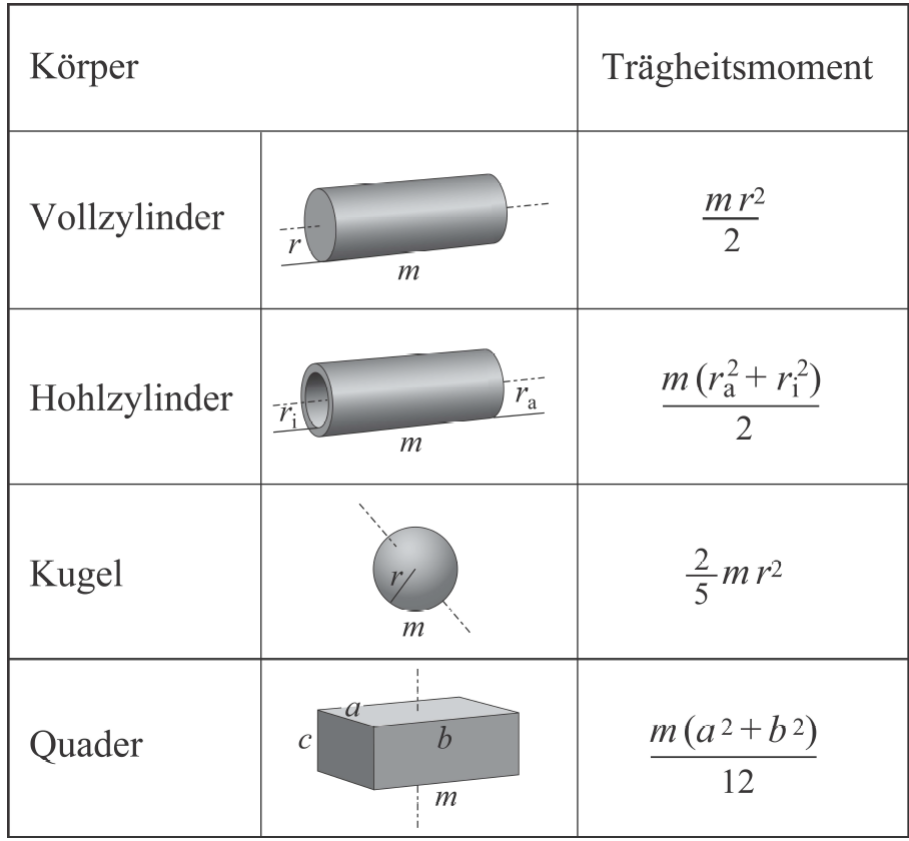
\includegraphics[width=0.75\linewidth]{images/Physik_1-Mechanik.png}


\subsection{Schweizer Strom-Mix}
$
\begin{array}{|c|l|}
    \hline
    38.1 \% & \text{Kernkraft} \\ \hline
    32.3 \% & \text{Speicherkraftwerke} \\ \hline
    24.2 \% & \text{Laufkraftwerke} \\ \hline
    5.4 \% & \text{konventionell-thermische Kraftwerke} \\ \hline
\end{array}
$

$
\begin{tabular}{|c|l|}
    \hline
    1.52 \% & Kehrichtverbrennungsanlagen \\ \hline
    0.29 \% & Biomasse \\ \hline
    0.19 \% & Abwasserreinigungsanlagen \\ \hline
    0.13 \% & Photovoltaik \\ \hline
    0.06 \% & Windkraft \\ \hline
\end{tabular}
$


\newcolumn
\subsection{Investitions- und Kostenrechnung}

\subsubsection{Annuitätsfaktor $A$}
$\boxed{A = \frac{(1 + i)^n \cdot i}{(1 + i)^n - 1}}$

\renewcommand{\arraystretch}{1.2} % Erhöht Zeilenhöhe für bessere Lesbarkeit
\begin{tabular}{@{} l p {4cm} l @{}}
    $[A]$       & Annuitätsfaktor           \dotfill & $1$ \\
    $[i]$       & Zinsen                    \dotfill & $1$ \\
    $[n]$       & Anzahl Jahre Laufzeit     \dotfill & $1$ \\
\end{tabular}


\subsubsection{Kapitalkosten $K_{\text{K}}$}
$\boxed{K_{\text{K}} = A \cdot I}$

\renewcommand{\arraystretch}{1.2} % Erhöht Zeilenhöhe für bessere Lesbarkeit
\begin{tabular}{@{} l p {4cm} l @{}}
    $[K_{\text{K}}]$    & Kapitalkosten     \dotfill & CHF oder € \\
    $[A]$               & Annuitätsfaktor   \dotfill & $1$ \\
    $[I]$               & Investitionen     \dotfill & CHF oder € \\
\end{tabular}


\subsubsection{Unterhaltskosten $K_{\text{U}}$}
$\boxed{K_{\text{U}} = p_{\text{U}} \cdot I}$

\renewcommand{\arraystretch}{1.2} % Erhöht Zeilenhöhe für bessere Lesbarkeit
\begin{tabular}{@{} l p {4cm} l @{}}
    $[K_{\text{U}}]$    & Unterhaltskosten              \dotfill & CHF oder € \\
    $[p_{\text{U}}]$    & Unterhaltskosten-Prozentsatz  \dotfill & $1$ \\
    $[I]$               & Investitionen                 \dotfill & CHF oder € \\
\end{tabular}


\subsubsection{Fix-Kosten $K_{\text{Fix}}$}
$\boxed{K_{\text{Fix}} = K_{\text{K}} + K_{\text{U}} = (A + p_{\text{U}}) \cdot I}$

\renewcommand{\arraystretch}{1.2} % Erhöht Zeilenhöhe für bessere Lesbarkeit
\begin{tabular}{@{} l p {4cm} l @{}}
    $[K_{\text{Fix}}]$    & Fix-Kosten              \dotfill & CHF oder € \\
\end{tabular}


\subsubsection{Erlös oder Deckungsbeitrag $E$}
$\boxed{E = t_{\text{VL}} \cdot C \cdot P}$

\renewcommand{\arraystretch}{1.2} % Erhöht Zeilenhöhe für bessere Lesbarkeit
\begin{tabular}{@{} l p {4cm} l @{}}
    $[E]$               & Erlös             \dotfill & CHF oder € \\
    $[t_{\text{VL}}]$   & Volllaststunden   \dotfill & $h$ \\
    $[C]$               & Grenzkosten       \dotfill & $\frac{\text{CHF}}{\text{MWh}}$ oder $\frac{\text{€}}{\text{MWh}}$ \\
    $[P]$               & Leistung          \dotfill & $W = \frac{Nm}{s} = \frac{J}{s}$ \\
\end{tabular}


\subsubsection{Ergebnis (Gewinn oder Verlust) $G$}
$\boxed{G = E - K_{\text{Fix}} - K_{\text{Var}}}$

\subsubsection{Variable Kosten $K_{\text{V}}$}

\renewcommand{\arraystretch}{1.2} % Erhöht Zeilenhöhe für bessere Lesbarkeit
\begin{tabular}{@{} l p {4cm} l @{}}
    $[G]$               & Ergebnis        \dotfill & CHF oder € \\
    $[E]$               & Erlös           \dotfill & CHF oder € \\
    $[K_{\text{Fix}}]$  & Fix-Kosten      \dotfill & CHF oder € \\
    $[K_{\text{Var}}]$  & Variable Kosten \dotfill & CHF oder € \\
\end{tabular}







































